%% LyX 2.3.7 created this file.  For more info, see http://www.lyx.org/.
%% Do not edit unless you really know what you are doing.
\documentclass[english]{article}
\usepackage[T1]{fontenc}
\usepackage[latin9]{inputenc}
\usepackage{babel}
\usepackage{array}
\usepackage{float}
\usepackage{textcomp}
\usepackage{amsmath}
\usepackage{amssymb}
\usepackage{graphicx}
\usepackage[unicode=true]
 {hyperref}

\makeatletter

%%%%%%%%%%%%%%%%%%%%%%%%%%%%%% LyX specific LaTeX commands.
\newcommand{\noun}[1]{\textsc{#1}}
%% Because html converters don't know tabularnewline
\providecommand{\tabularnewline}{\\}

\makeatother

\begin{document}
\title{\textbf{Study of Josephson Junction fabrication and characterisation
}\\
}
\author{\noun{Undergraduate Thesis}}
\author{\medskip{}
\\
Submitted in partial fulfillment of the requirements of\emph{}\\
\emph{BITS F421T Thesis }\\
\emph{By} \\
Ashwin Kumar K\\
ID No. 2017B5A81034G\\
\medskip{}
\\
\emph{Under the guidance of :}\\
\medskip{}
\\
Dr. Kartik Senapati, NISER, Bhubaneswar\\
\emph{\&}\\
Dr. Ram Shanker Patel, BITS Pilani, Goa}

\maketitle
\begin{figure}[H]

\begin{centering}
\includegraphics[width=5cm]{bits_logo}
\par\end{centering}
\end{figure}

\newpage{}

\section*{Declaration}

I, Ashwin Kumar K, declare that this Undergraduate Thesis titled, `Study of Josephson Junction fabrication and characterisation' and the work presented in it are my own. I confirm that:
\begin{itemize}     \item[\tiny{$\blacksquare$}] This work was done mainly or wholly  while in         candidature for a research degree at this University.     \item[\tiny{$\blacksquare$}] Where any part of this thesis has previously         been submitted for a degree or any other qualification at this         University or any other institution, this has been clearly stated.     \item[\tiny{$\blacksquare$}] Where I have consulted the published work of         others, this is always clearly attributed.     \item[\tiny{$\blacksquare$}] Where I have quoted from the work of others,         the source is always given. With the exception of such quotations, this         thesis is entirely my own work.     \item[\tiny{$\blacksquare$}] I have acknowledged all main sources of help.     \item[\tiny{$\blacksquare$}] Where the thesis is based on work done by         myself jointly with others, I have made clear exactly what was done by         others and what I have contributed myself.\\ \end{itemize}
Signed:\\ \rule[1em]{25em}{0.5pt} % This prints a line for the signature
Date:\\ \rule[1em]{25em}{0.5pt} % This prints a line to write the date     }

\newpage{}

\section*{Acknowledgements}

I wish to thank my project supervisors, Dr. Kartikeswar Senapati and
Dr. Ram Shanker Patel for their immense support and help with the
understanding of this project. I would like to express my deepest
appreciation to Mr. Tapas Ranjan Senapati and Ms. Laxmipriya Nanda
for all their help from mentoring on the fabrication techniques to
usage of measurement systems and all the fruitful discussions. I wish
to thank all the lab members of Superconductivity lab, NISER for all
the brainstorming sessions which helped me greatly. Special thanks
to Ms. Soheli Mukherjee who always supported me with all my endeavours.
I would also like to extend my deepest gratitude to Dr. Dhavala Suri
who always showered me with helpful advice. lastly, I am thankful
to all my friends and family members for extending their love and
support.

\newpage{}

\tableofcontents{}

\section*{\newpage}

\section*{Abbreviations}
\begin{itemize}
\item AC :- Alternating current 
\item RF :- Radio frequency 
\item JJ :- Josephson Junction
\item SQUID :- Superconducting QUantum Interference Device
\item EDX :- Energy Dispersive X-ray spectroscopy 
\item SEM :- Scanning Electron Microscope
\item FIB :- Focused Ion Beam 
\item PPMS :- Physical Properties Measurement System 
\item Fig :- Figure 
\item eV :- Electron Volt 
\item KeV :- Kilo Electron Volt 
\item MeV :- Mega/Million Electron Volt 
\item et al :- And others (Latin) 
\item i.e. :- That is 
\item etc :- Et cetera (Latin for \textquoteright and others of same kind\textquoteright ) 
\item T :- Tesla 
\item SiO2:- Silicon dioxide
\item R-T :- Resistance Versus Temperature 
\item I-V :- Current Versus Voltage 
\item I-H :- Current Versus Magnetic field 
\item V-H :- Voltage Versus Magnetic field 
\item Si :- Silicon 
\item K :- kelvin
\item mm :- millimeter 
\item mbar :- millibar 
\item IPA :- Isopropyl alcohol 
\item RPM :- Revolutions Per Minute 
\item C :- Celsius 
\item Ar :- Argon 
\item e.g. :- Example given 
\item TSP :- Titanium Sublimation Pump 
\item RGA :- Residual Gas Analyzers 
\item Cu :- Copper 
\item BCS :- Bardeen--Cooper--Schrieffer 
\item Nb :- Niobium 
\item DC :- Direct current
\item AC :- Alternating current
\item $\mu$A :- Micro Ampere 
\item $\Omega$:- Ohm 
\item nm :- Nano meter
\end{itemize}
\newpage{}

\part{Introduction}

At the beginning of this thesis, we introduce basic theoretical concepts
that underlay the device we are trying to study, i.e. the Josephson
Junction (JJ). We first study the postulates of superconductivity.
Then we look at the Josephson effect, which describes the physics
of a Superconductor-Insulator-Superconductor sandwich and then look
at a popular model of a realistic Josephson junction, namely the RCSJ
model. Later we will try to understand various aspects of fabrication
and characterisation of such devices.

\section{Superconductivity}

Heike Kamerlingh Onnes discovered the phenomenon of superconductivity
in the Netherlands in 1911. He was the first to observe that the electrical
resistance becomes exactly zero in certain materials and in temperatures
below a specific critical value $T_{c}$ \cite{Tinkham-1}. Soon after
this discovery, several other materials that showed superconducting
behaviour were discovered, with different critical temperatures. Currently
the highest temperature at which superconductivity was observed is
in hydrogen sulphide ($H_{2}S$), which has a $T_{c}$ reported as
203K, but at extremely high pressures \cite{HighTc}. In 1933, Meissner
and Ochsenfeld discovered that within a superconductor, the magnetic
field completely vanishes i.r becomes zero, making the superconductor
a perfect diamagnet. The expulsion of a magnetic field inside a superconductor
is called the Meissner effect. Then the London brothers explained
this effect, who proved that the magnetic field inside a superconductor
has an exponential decay from the surface, with a decay length $\lambda$,
called London penetration depth. They explained that in order to facilitate
this, the superconductor sets up electric currents on its surface,
whose magnetic field opposes and cancels the applied magnetic field
within the superconductor. The phenomenon of superconductivity was
theoretically explained in 1957, almost 46 years after its initial
discovery, by Bardeen, Cooper, and Schrieffer \cite{BCS}. They proposed
the first microscopic theory of superconductivity, which was named
the BCS theory, and received the Nobel Prize in Physics in 1972. They
suggested that the electrons of a superconductor that are close to
the Fermi surface attract indirectly through the crystal lattice,
which is mediated by the exchange of phonons. This attraction overcomes
the Coulomb repulsion between the two electrons and the electrons
form pairs, which we now call as Cooper pairs. Cooper pairs feel no
scattering, and thus lead to the formation of supercurrent. In $T>T_{c}$
though, the thermal vibration energy of the lattice becomes more significant
than the pairing energy of the electrons, so the Cooper pair breaks,
and thus the material becomes normal. It was later discovered that
superconducting materials behave in different ways upon application
of external magnetic fields. There are two major categories of superconductors
which are type I and type II. A type I has only one critical field
(keeping other parameters like current density and temperature constant)
above which all superconductor properties are lost and while in superconducting
state all magnetic field lines or magnetic flux are completely pushed
out from the bulk of the material. In the case of a type II superconductor,
there exists two separate critical field values between which a single
flux quanta, $\phi_{0}$, of the magnetic field is allowed to pass
through the superconductor through isolated points and are called
vortices. Currently one of the most used applications of superconductivity
is to produce extremely high magnetic fields ranging into tens of
teslas can trace it\textquoteright s origin back to 1955 when G. B.
Yntema created the first ever superconducting electromagnet using
superconducting Nb wire windings with an iron-core, this setup was
outputting a 0.7 T magnetic field

\section{Josephson Junctions}

Prior to 1962, researchers were familiar with quantum mechanical tunnelling
of normal electrons through a weak barrier; however, the probability
of tunnelling of a cooper pair was thought to be insignificant given
that the pair as a whole would have to tunnel through the barrier.
In 1962 Brian David Josephson showed that this tunnelling probability
is not low as previously thought. He predicted theoretically that
two superconductors that are coupled (are in close proximity) by a
weak link, which link may be made of a normal metal, an insulator,
or a constriction of superconductivity, can still let the supercurrent
flow through them \cite{BDJJ}. This macroscopic phenomenon was given
the name Josephson effect. 
\begin{figure}[H]
\centering{}\includegraphics[width=8cm]{a-The-superconducting-order-parameter-of-a-superconductor-S-penetrating-into-the}\caption{(a) The superconducting order parameter $\Psi$ of a superconductor
(S) penetrating into the normal metal (N) with a length scale of the
superconducting coherence length,$\xi$. (b) Order parameters from
two sides have an overlap in N, producing proximity Josephson coupling.\cite{SCFig}}
\end{figure}

Josephson demonstrated that, for a short junction, the current that
flows through the junction when no voltage bias is applied, and the
phase difference $\phi$ across the junction, which is the difference
in the phase factor between the order parameter of the two superconductors,
are related through the relation: 
\begin{equation}
I_{s}=I_{c}\,sin(\delta)\label{eq:JJ1}
\end{equation}
 Here, $I_{c}$ is the supercurrent amplitude and $\delta=\phi_{1}-\phi_{2}$
, where $\phi_{i}$ is the phase of each superconductor. This phenomenon
is known as the DC Josephson effect. Josephson also showed AC Josephson
effect where an applied constant voltage bias V on the junction leads
to sinusoidal oscillations in the junction current and is governed
by the equation: 
\begin{equation}
V=\left(\Phi_{0}/2\pi\right)\dot{\delta}\label{eq:JJ2}
\end{equation}
 where $\Phi_{0}\approx2\times10^{-15}$ Weber is the flux quantum.

The DC Josephson effect is explained by a process known as Andreev
reflection \cite{Tinkham-1}. A.F.Andreev explained the phenomenon
in 1964 establishing the concept of the so-called Andreev reflection
This reflection occurs at the interfaces between the superconductor
S and a normal metal N. Andreev suggested that an electron that approaches
the interface from the normal metal side can travel through the superconductor
side by the formation of a Cooper pair with another electron with
opposite momentum and spin on the superconductor side. At the same
time, reflect a hole inside the normal metal region thus balancing
the charge. As a result of this cycle, a pair of correlated electrons
is transferred from one superconductor to another, creating a supercurrent
flow across the junction. It explains how a normal current in the
normal metal side becomes a supercurrent in the superconductor side.
The AC Josephson relation in essence suggests that a Josephson junction
can be a perfect voltage-to-frequency converter. The inverse is also
possible by using a microwave frequency to induce a DC voltage in
a Josephson junction, this phenomena is known as inverse AC Josephson
effect.

\begin{figure}[H]
\centering{}\includegraphics[width=5cm]{andreev_reflection}\caption{Andreev Reflection process}
\end{figure}


\subsection{RCSJ model}

A Josephson junction, is typically composed of two superconducting
electrodes separated by weaklink which is typically insulating, thus
such a junction would have some unavoidable capacitance $C$ (Just
like the parallel plate capacitor separated by a dielectric). If the
junction current exceeds the critical current of the junction then
quasi-particle excitations are generated. These quasi-particle currents
are not superconducting and can be quite lossy just like a normal
metal current, so we represent this as a normal resistor $R$. This
gives us the resistively and capacitivly shunted junction (RCSJ) model.
This model helps us simulate the characteristics of a Josephson junction.
A schematic representation of the same can be seen in Fig \ref{fig:Schematic-of-RCSJ}.

\begin{figure}[H]
\centering{}\includegraphics[width=5cm]{RCSJ}\caption{A schematic representation of RCSJ model. Here $I$ is the current
through the device, $I_{c}$ is the current through the capacitor
$I_{J}$ is the current through the Josephson Junction, $I_{R}$ is
the current through the resistance\label{fig:Schematic-of-RCSJ}}
\end{figure}

Writing out Kirchov's circuit laws for the RCSJ model (from Fig \ref{fig:Schematic-of-RCSJ}.)we
can find 

\[
I_{c}+I_{J}+I_{R}=I
\]

\[
\frac{\Phi_{0}}{2\pi}C\ddot{\delta}+I_{c}\sin(\delta)+\frac{\Phi_{0}}{2\pi R}\dot{\delta}=I
\]

or
\[
\frac{\Phi_{0}}{2\pi}C\ddot{\delta}+\frac{\Phi_{0}}{2\pi R}\dot{\delta}=I-I_{c}\sin(\delta)
\]
 Rearranging as 
\begin{equation}
\ddot{\delta}+\frac{1}{RC}\dot{\delta}=\left(\frac{2\pi}{C\Phi_{0}}\right)\left(I-I_{c}\sin(\delta)\right)\label{eq:dammpedeqn}
\end{equation}
 we can interpret Eq \ref{eq:dammpedeqn} as the dynamics of a damped
particle with the following physical properties:
\[
\begin{aligned}\text{ "effective mass" } & =C\\
\text{ "coefficient of friction" } & =1/R\\
\qquad\text{ "potential experienced by the particle" } & =-\left(2\pi/C\Phi_{0}\right)\left(I\delta+I_{c}\cos(\delta)\right).
\end{aligned}
\]

The dynamics of the Josephson junction phase difference in-terms of
the damped particle can be described as follows: (Fig \ref{fig:washboard-potential})

\begin{figure}[H]
\centering{}\includegraphics[width=13cm]{JJ-IV}\caption{Interpretation of the washboard potential\cite{JJ-IVexpln}\label{fig:washboard-potential}}
\end{figure}

\begin{itemize}
\item When there is no junction current (at I=0) the junction experiences
a purely cosine potential. At this stage the pseudo-particle sits
trapped in one of the wells of the cosine, as indicated in Fig \ref{fig:washboard-potential}a.
As we introduce some current we see the effect of an added linear
term to the potential. The potential now resembles a tilted washboard,
and hence is called as the \emph{tilted washboard potential}. If the
bias current is less than $I_{C}$ there are still vallies in the
potential and the ball remains trapped as indicated also in Fig \ref{fig:washboard-potential}a.
Because the junction phase (i.e the pseudo-particle) is stuck at a
fixed value of $\delta$, the voltage is zero (as $V\propto\dot{\delta}$
). This is the part of the IV curve where increase in junction current
does not lead to increase in the junction voltage, as indicated in
the horizontal blue line. At this stage since the junction element
is still superconducting, all of the current flows through the tunnel
element and none flows through the resistor thus the junction .
\item As we increase the current past $I_{c}$, the linear term in the potential
dominates the cosine part and the vallies start to disappear. The
junction pseudo particle then rolls down hill as shown in Fig \ref{fig:washboard-potential}b.
The pseudo particle now experiences a time varying phase, thus the
junction voltage becomes non-zero and reaches to a finite value, this
can be seen in the red line in Fig \ref{fig:washboard-potential}b
\item Now, the current I exceeds the critical current of the tunnelling
element and so the tunnelling element no longer behaves as a superconductor.
Quasiparticles are generated, rendering the junction resistive. In
other words nearly all of the current flows through the resistive
element. Further increases in current show an accompanying linear
increase in voltage according to $V=IR$, similar to that of a normal
metal as shown in Fig \ref{fig:washboard-potential}c, and by the
green line marked Fig \ref{fig:washboard-potential}c.
\item As the current is lowered, we travel back down the green line, as
indicated by the mark Fig \ref{fig:washboard-potential}d. The rest
of the process depends on how fast we are raising and lowering the
current. As we lower the current below $I_{c}$, the potential regains
its cosine nature and regains vallies.
\item If there were no dissipative forces as is the case when we sweep fast
enough or when whatever dissipation remains can't completely stop
the particle, the particle would continue to roll down as it already
has energy. Therefore, even as I is lowered below $I_{c}$ we still
have time varying $\delta$ and therefore still have a measurable
voltage. This can be concluded from Fig \ref{fig:washboard-potential}e
and the pink line in Fig \ref{fig:washboard-potential}e 
\item In the end, we go back to no bias case where the potential is again
a cosine term and as we slowly sweep the voltage we slow down and
finally stop the particle. Then as we increase the negative bias the
process starts all over in reverse.
\end{itemize}

\subsection{Josephson Junctions in the Presence of a Magnetic Field}

In Eq\ref{eq:JJ1} we saw that he Josephson Junction current depends
on the phase difference $\delta$ across the junction. When an external
magnetic field is applied, the field influences the phase difference
$\delta$, this in turn causes interesting dynamics between the Josephson
Junction current and the applied external magnetic fields. It can
be shown that in the case of a small Josephson Junction this dependence
follows the relation\cite{Tinkham-1}: 
\[
I_{J}=I_{0}\left|\frac{\sin\left(\pi\frac{\Phi_{J}}{\Phi_{0}}\right)}{\pi\frac{\Phi_{J}}{\Phi_{0}}}\right|
\]

here $\Phi_{J}=\mu_{0}HLd\text{ is the magnetic flux linked to the whole barrier }$.
This is the standard from of the Fraunhofer pattern $F(x)=I_{0}\sin^{2}(\pi x)/(\pi x)^{2}$and
is seen as a unique characteristic confirmation of a Josephson junctions.
For a SQUID, the critical current-magnetic field characteristic is
similar to that of Josephson Junctions with the addition of SQUID
oscillations superimposed on it. Both of these signatures are verified
experimentally for the devices fabricated in lab in later sections.

\newpage{}

\part{Experimental Details}

\section{Sample preparation}

For our Josephson junction device we chose the superconductor as Niobium
and the weaklink as Copper, based on availability of sputter targets
in the lab. These devices were prepared on a 5 x 5 $mm^{2}$ $Si/SiO_{2}$
substrate cut from a $Si/$$SiO_{2}$ wafer. The substrates were cleaned
with acetone and trichloroethylene both of which are de-greasing agents
and IPA which removes any strains left from acetone, followed by DI
water bath to remove the residue of the $SiO_{2}$ or Si on the substrates.
Each process was carried out with ultrasonication for 5 minutes in
a cleaned beaker. the substrates were then cleaned with the compressed
air along with Some IPA in it. The air gun pressure was maintained
at 4 PSI. We tried our best to minimise the interface roughness of
the sample and to grow the thin-film uniformly.

In order to confirm the presence of magnetic moment in the presence
of a SOC material at the weaklink of Josephson Junction and SQUID,
we wanted to make Pt/Cu/Nb planar junction ( and SQUID ) where Pt
is the bottom layer. We also wanted to observe the effect of varying
thickness of the platinum layer and the copper layer. All the samples,
thus essentially contain three layers : Nb (155nm), Cu ( varying between
30nm to 100nm), Nb (155nm). For planar Josephson junction the third
layer made of Niobium was absent. For all of our requirement we optimized
all the thickness of the material before using in trilayer study or
making devices. All the instruments apart from the deposition system
used in the fabrication process were used inside a clean room. 

\section{Lithography}

For device fabrication like, planar Josephson junction and planar
SQUIDS, we need a 2$\mu m$ width line made of Nb/Cu/Pt trilayer.
For optimizing thickness and do the characterisation for all the layers
individually, we did it on same 2$\mu m$ width track. The patterns
were made with the mask aligner lithography machine (Midas MDA-400M)
followed by a high precession speed controlled Spin coater.

In order to make the 2$\mu m$, we used photo lithography process
with a pre-made mask. The mask contains the 2$\mu m$ line along with
lines drawn on the contact pad at regular intervals. This allows us
to make 7 devices at a time on the same sample. An image of the mask
is shown in Fig \ref{fig:mask}.

\begin{figure}
\centering{}\includegraphics[width=5cm]{pattern}\caption{Image of the mask that was used for lithography\label{fig:mask}}
\end{figure}

\begin{figure}
\centering{}\includegraphics[width=5cm]{maskAligner}\caption{Image of the mask aligner that was used for lithography\label{fig:mask-1}}
\end{figure}

For the photo lithography process, $Si/$$SiO_{2}$wafer was cut in
to several 5mm x 5mm substrate. after cleaning the substrates in the
above mentioned process, a uniform layer of PMMA (+ve ) Photoresist
was applied to the clean substrates and then spun rapidly using a
spin coater at 3000 RPM to even out the photoresist layer, and then
baked at 70$^{\circ}$C for 1 minute to evaporate the solvent. After
the photoresist was applied, the mask was placed on Mask aligner and
was exposed to the UV light for 30s to weaken the photoresist on the
exposed area. Since these trilayer height were more than 300nm, there
were difficulties while doing the liftoff process. The stress on the
bottom layer creates an slanted edge on track. So while liftoff there
is some possibilities that the 2$\mu m$ line come out because of
the stress from outside photoresist. To avoid these circumstances
we used the undercut process in the lithography, the undercut process
helps us in making the photoresist edge in a convex shape as shown
in Fig\ref{fig:The-different-profiles}. Which would help us to make
a discontinuity in the track height thus easing the liftoff process.
\begin{figure}
\centering{}\includegraphics[width=10cm]{photo-resist}\caption{The different profiles achieved with (a) a single layer of resist,
(b) resist soaked in chlorobenzene for few seconds and (c) a bilayer
of electron sensitive resist \label{fig:The-different-profiles}\cite{undercutImage}}
\end{figure}
 In the case of a positive photoresist, the UV radiation exposed region
of the photoresist becomes soluble in the developing solution (Sodium
hydroxide solution). After the developing, the photoresist forms a
negative image of the required pattern.

Image taken from optical microscope of the sample after the photolithography
process is shown in Fig \ref{fig:Litho1}. One can clearly see the
part where the photoresist is present (yellowish in colour) and where
the photoresist is absent ( due to the $Si/$$SiO_{2}$substrate below).

\begin{figure}
\centering{}\includegraphics[width=5cm]{litho1}\caption{Image taken from optical microscope of the sample after the photolithography
process \label{fig:Litho1}}
\end{figure}

During deposition, the material would cover these gaps and upon liftoff
the material deposited on the photoresist would go away along with
the resist leaving just the material at the desired place as shown
in Fig \ref{fig:Litho2}. 

\begin{figure}
\centering{}\includegraphics[width=5cm]{Litho2}\caption{Image taken from optical microscope of the sample after deposition
and liftoff process \label{fig:Litho2}}
\end{figure}


\section{Deposition }

Pt/Cu/Nb trilayer films were prepared on patterned substrates at ambient
temperature using DC-magnetron sputtering with high purity (99.99\%)
Pt,Cu and Nb targets. The DC-magnetron sputtering system present in
superconductivity lab, NISER is shown in Fig \ref{fig:The-DC-magnetron-sputtering}. 

The base pressure of the deposition chamber was of the order of $10^{-9}$mBar.
At normal temperatures standard vacuum chambers have a tendency of
holding $H_{2},H_{2}O$ and CO molecules by physical adsorption at
the inner surface of the chamber and could take hours before they
are pumped outside. By baking the chamber walls to 150$^{\circ}$C
for about 12hrs and then cooling the contaminants could be pumped
out further. A Residual Gas Analyser (RGA) was used to measure the
pressure of contaminants. RGA is a small mass spectrometer typically
used for contamination monitoring in vacuum systems. The RGA is able
to effectively determines the chemical composition of the residual
gas within the vacuum chamber, it works by ionising the residual gases
present in the chamber to create ions of these gas molecules before
determining their mass-to-charge ratio. It has a working range from
$\approx5\times10^{-2}$ mbar to $5\times10^{-8}$ mbar.

\begin{figure}[H]
\centering{}\includegraphics[width=10cm]{Sputter-Coater}\caption{The DC-magnetron sputtering setup present in superconductivity lab,
NISER \label{fig:The-DC-magnetron-sputtering}}
\end{figure}
The typical pressure of $N_{2},O_{2},H_{2}O$ in $10^{-8}mBar$ are
3,3,3.5. If the contaminant pressure is more than this base line,
Titanium Sublimation pump (TSP) is used as many times as need to obtain
the base line. A TSP works by heating a titanium filament wire to
about 1300$^{\circ}$C by passing about 40A current for a minute.
TSP is a type of vacuum pump used to remove residual gases in ultra-high
vacuum systems. It has a titanium filament, when a sufficiently high
current is passed, the filament reaches the sublimation temperature
of titanium and which causes the surrounding walls of the vacuum chamber
to gets coated with a layer of clean titanium. Due to the highly reactive
nature of titanium, the gas molecules that collides with the titanium
coated chamber walls are likely to chemically react with the titanium
to form a stable, solid product. Thus reducing the gas pressure in
the chamber. Pure Argon was then introduced to the chamber via a mass
flow controller at the rate of 20SCCM. The argon helps in initiating
the argon plasma across the target. The energetic ions are accelerated
towards the target. The ions strike the target and atoms are ejected
(or sputtered) from the surface. To initiate plasma generation, high
voltage of constant power is applied between the cathode ( located
directly behind the sputtering target ) and the anode (which is also
connected to the chamber as electrical ground). Electrons which are
present in the sputtering gas are accelerated away from the cathode
causing collisions with nearby atoms of sputtering gas. These collisions
cause an electrostatic repulsion which \textquoteleft knock off\textquoteright{}
electrons from the sputtering gas atoms, causing ionization. The positively
charged sputter gas atoms are now accelerated towards the negatively
charged cathode, leading to high energy collisions with the surface
of the target. Each of these collisions can cause atoms at the surface
of the target to be ejected into the vacuum environment with enough
kinetic energy to reach the surface of the substrate. In order to
facilitate as many high energy collisions as possible -- leading
to increased deposition rates -- the sputtering gas is typically
chosen to be a high molecular weight gas such as argon or xenon. Strong
magnets behind the cathode is used to confine the electrons in the
plasma at or near the surface of the target. Confining the electrons
leads to a higher density plasma and increased deposition rates. The
target is cooled by water so that the heat generated will not build
up to effect the magnets which keeps the plasma from spreading Shutter
plates made of stainless steel is placed in front of target with a
narrow opening in order to further improve the deposition. The sample
stage is slowly rotated such that the substrates get slowly exposed
to the plasma via the shutter plate opening thus enabling even deposition.
The height from the substrate plate to the target, the plasma power,
the plasma ignition pressure and the argon flow rate are all optimised
for each material, previously for good quality deposition. Shutter
plate opening width and sample stage rotation speed is optimised for
deposition thickness for each target. The following table summarises
the various optimisation parameters for the three targets:

\begin{table}[H]
\centering{}%
\begin{tabular}{>{\raggedright}p{0.07\textwidth}>{\centering}p{0.12\textwidth}>{\raggedright}p{0.12\textwidth}>{\raggedright}p{0.12\textwidth}>{\raggedright}p{0.12\textwidth}>{\raggedright}p{0.12\textwidth}>{\raggedright}p{0.12\textwidth}}
\hline 
Target & Sputtering pressure & Height of substrate from target & Plasma power & Argon flow rate & Shutter plate opening width & Sample stage rotation speed\tabularnewline
\hline 
Nb & 
\[
1.08x10^{-2}mbar
\]
 & 30 mm & 55 W & 20SCCM & 25.2 degree & 0.06 deg/min for 155nm\tabularnewline
Cu & 
\[
1.08x10^{-2}mbar
\]
 & 30 mm & 50 W  & 20SCCM & 10.8 degree & 0.1 deg/min for 100nm\tabularnewline
Pt & 
\[
1.08x10^{-2}mbar
\]
 & 30 mm & 50 W & 20SCCM & 10.8 degree & 1 deg/min for 20nm\tabularnewline
\hline 
\end{tabular}\caption{Optimisation parameters for different targets}
\end{table}


\section{Fabrication geometry }

Once the trilayer has been deposited and liftoff is done, we need
to form the trilayer into the Josephson junction geometry. Josephson
Junctions are typically fabricated via shadow deposition wherein a
floating mask and angled deposition creates valleys such that the
top and the bottom layers can be accessed separately. After the first
angled deposition, controlled oxidation of the first layer leads to
the formation of a very small insulating barrier. A schematic process
diagram of the shadow deposition technique is shown in Fig \ref{fig:The-shadow-deposition}.

\begin{figure}[H]
\centering{}\includegraphics[width=7cm]{shadow-dep}\caption{The shadow deposition technique for Josephson Junction fabrication
\cite{JJfab}\label{fig:The-shadow-deposition}}
\end{figure}

Another way to get to the required geometry is to use a subtractive
manufacturing process like a Focused Ion Beam (FIB). A FIB is similar
to and SEM in that it uses a beam of ions to image and directly modify
or \textquotedbl mill\textquotedbl{} the specimen surface via the
sputtering process. This milling can be controlled with nanometer
precision. Crossbeam 340 from ZEISS, which uses gallium ions for the
FIB is available in NISER and was used extensively for the fabrications
of the Josephson junction samples. The Crossbeam 340 has a FESEM and
gallium FIB guns mounted at $54^{\circlearrowleft}$ to each other.
The sample and the stage is adjusted such that the focal axis of both
FIB and SEM co-inside at the surface of the sample and is at a working
distance of 5.12mm away from the gun tip. This alignment shown in
Fig \ref{fig:Alignment-of-SEM} ensures that the imaging done by the
SEM and the milling done by the FIB co-inside. 
\begin{figure}[H]
\centering{}\includegraphics[width=7cm]{secondRenderY}\caption{Alignment of SEM gun (grey) and FIB gun (brown) axis at the surface
of the sample (purple) mounted on the stage (silver) \label{fig:Alignment-of-SEM}}
\end{figure}
 While milling, highly energised gallium ions strike the sample causing
the target to sputter atoms from the surface. In this process gallium
atoms will get embedded in the top few nano meters of the target surface,
and the surface will become amorphous, this is known as gallium poisoning.

There are two geometries in which the Josephson junction are fabricated
using FIB, one is the vertical Junction (Fig \ref{fig:Vertical}),
and the other is the planar Junction (Fig \ref{fig:Planar}); both
names describe the path the current takes through the trilayers. In
the planar Junction, the current is in plane with the trilayers and
in the case of the vertical junctions the current flows vertically
through the trilayers. 

\begin{figure}[H]
\centering{}\includegraphics[width=6cm]{JJ-planar}\caption{Schematic of the Planar Josephson Junction, due the vertical FIB cut
in the Niobium layer, the current travels in plane through first the
Niobium layer then through the copper weaklink then finally through
the other Niobium layer. The yellow arrowed line shows the direction
of current flow\label{fig:Planar}}
\end{figure}

\begin{figure}[H]
\centering{}\includegraphics[width=6cm]{JJ-verical}\caption{Schematic of the Vertical Josephson Junction, due to the nano pillar
cuts on the left and the right, the current travels in plane through
first the top Niobium layer then through the copper weaklink then
finally through the other Niobium layer. The yellow arrowed line shows
the direction of current flow\label{fig:Vertical}}
\end{figure}

In order to do the Planar, cut the stage was tilted in such a way
that the sample is perpendicular to the FIB gun, similar to the arrangement
in Fig \ref{fig:Alignment-of-SEM}. Then a vertical cut is made to
a controlled depth.In order to control the depth of the cut, exposure
time had to be optimised. This was done by cutting several vertical
lines away from the 2$\mu$ line with varying exposure time. Then
Energy Dispersive Spectroscopy (EDAX) was done on these multiple cuts
to see which exposure time first cuts the Niobium layer and thus exposing
the Copper below it (Fig \ref{fig:Edax}). 
\begin{figure}[H]
\centering{}\includegraphics[width=7cm]{Edax}\caption{Energy Dispersive Spectroscopy (EDAX) of the multiple vertical cuts
done in order to optimise the FIB cutting depth \label{fig:Edax}}
\end{figure}
 The basic principle of EDAX is as follows: During SEM microscopy,
the primary electron beam sometimes removes electrons from the inner
shells of an atom causing the outer electron to jump into the vacant
spot by releasing energy in the form of X-rays. This energy difference
is unique for each element and the element can be identified from
it\textquoteright s characteristic X-ray. EDS measures these characteristic
X-rays thus identifying the chemical composition of the sample.

An image of the sample after milling with FIB as seen through an optical
microscope is shown in Fig .

\begin{figure}[H]
\centering{}\includegraphics[width=5cm]{Litho-3}\caption{Image taken from optical microscope of the sample after milling with
FIB, the devices are encircled\label{fig:Litho3}}
\end{figure}


\section{Wire bonding}

After the sample is prepared, electrical connections need to be made
for sending current, measuring voltage,etc. For this a wire bonding
apparatus is used which uses 50$\mu m$ dia silicon doped aluminium
wires for the connections. The needle through which the aluminium
wire comes through, embeds the wire in the sample by vibrating at
ultrasonic frequencies.

Ultrasonic bonding was discovered 1960 through a several experimental
observation and has subsequently been developed into a highly controlled
process. In recent years it has been used extensively for electrical
interconnecting of semiconductor chips in the semiconductor fabrication
industry and in material science research laboratories for making
reliable conducting contacts on sample and pucks. There are four types
of wire bonding:
\begin{description}
\item [{Thermocompression~Bonding}] A process which involves the use of
force, time, and heat to join the two materials by inter- diffusion.
This process uses gold wire.
\item [{Gold~Ball~Bonding}] Uses gold wire ultrasonicated at the surface
to make the ball. This process uses heat force, time, and ultrasonics.
\item [{Wedge~Bonding}] This process uses aluminium wire formed below
a narrow metalic wedge. The wedge forces the wire on top of the sample
and ultrasonicates therby making a metallic bond between aluminium
and the sample. No heat is required in this process. This process
is the one used all the sample preparation in regards to the current
thesis.
\item [{Thermosonic~Bonding}] This requires gold wire and capillaries.
This process uses force, time. heat, and ultrasonics to make a ball.
This process is accomplished by melting the wire to form a ball.
\end{description}

\subsection{Wedge Bonding}

Ultrasonic energy, when applied to metallic wire to be bonded, renders
it temporarily soft and plastic. This causes the metal to flow under
pressure. The acoustic energy frees the dislocation from their pinned
positions which allows the metal to flow under the low compressive
forces of the bond. Thus heat at the bond becomes a byproduct of the
bonding process, and the heat becomes unnecessary to form the bond.
The deformation of the wire will break up and sweep aside the contaminants
in the weld area. This exposes extremely clean metallic surfaces which
promotes the metallurgical bonds.

In wedge bonding, the wire come out through a 50 $\mu m$ hole at
45� angle and then under the needle tip which is shaped like a wedge
as seen in Fig \ref{fig:Image-of-wire}. 

\begin{figure}[H]
\centering{}\includegraphics[width=5cm]{\string"wedge tip\string".eps}\includegraphics[width=2.5cm]{\string"wedge tip2\string".eps}\caption{Image of wire threaded through the wedge shaped needle. The left image
clearly shows the wedge shape and the right is a cross section image
showing how the needle is threaded.\cite{wirebonder} \label{fig:Image-of-wire} }
\end{figure}

The quality of wire bonded is also sensitive to the height between
the base plate and the needle tip when it is bonding, the wirebonder
at NISER is setup such that this effective height is 76mm, at this
height ultrasonic power and the bonding force are most effective,
because the transducer is in surface and the bond tool stands perfectly
vertical. Therefore the distance from base plate should always be
fixed to this value.

In case the Surface is higher, the bond will be affected when the
tool touches the surface. At a surface height >78 mm the ultrasonic
power and bonding force are less effective and most probably the parameters
have to be increased. If the bonding surface is lower than 76 mm,
the bond will be automatically activated at a height of 75.5 mm, even
if the tool does not touch the surface. So it is impossible to bond
at a lower height. The steps involved in making the two bonds are
shown in Fig \ref{fig:wirebondersteps}.

\begin{figure}[H]
\centering{}\includegraphics[width=10cm]{\string"Wedge bonding process\string".eps}\caption{The steps involved in making a bond from the puck to the contact pads
on the sample \cite{wirebonder}\label{fig:wirebondersteps}}
\end{figure}

A principle disadvantage of wedge bonding is the wire is fed at a
45� or 60� horizontal angle rather than perpendicular as in ball bonding.
Also, wedge bonding is unidirectional.

This is slower than ball bonding which is multidirectional. Wedge
bonding requires the circuit workpiece or the bonding head to rotate
to allow for the wire to bond in the appropriate direction.

\begin{figure}[H]
\centering{}\includegraphics[width=10cm]{wedgeboding-surface}\caption{Image of a bond site which was done by wedge bonding tool. \cite{wirebonder}\label{fig:wirebondersteps-1}}
\end{figure}


\section{Characterization}

\subsection{Physical Property Measurement System (PPMS)}

In order to do analysis/characterisation of any material/nano device,
one typically need measurement of several physical properties of DUT.
Typical physical characteristics like, 
\begin{itemize}
\item Resistance as a function of temperature
\item Current voltage characteristics
\item Magnetic susceptibility as a function of applied external magnetic
field (VSM)
\item Magnetoresistance
\item Other transport measurements like specific heat, magnetic AC and DC
susceptibility and both electrical and thermal transport properties
(like Hall Effect, thermoelectric figure of merit and Seebeck Effect)
etc.
\end{itemize}
are most often used to characterise bulk and thinfilm samples. Superconductivity
lab, NISER has a PPMS setup by Cryogenics that allows one to do low
temperature characterisation of materials (1.6K - 300K) at different
magnetic fields (upto 9 Tesla) and under different electric configuration
of the sample. Fig\ref{fig:PPMS} shows the image of the PPMS system
present in the lab. 
\begin{figure}[H]
\centering{}\includegraphics[width=5cm]{PPMS}\caption{Image of the PPMS system present at Superconductivity lab NISER\label{fig:PPMS}}
\end{figure}

The setup comprises of the following main components:
\begin{itemize}
\item A cryostat incorporating a cryocooler, superconducting magnet and
a variable temperature sample space.
\item Rack incorporating electronics for control and monitoring of the cryostat
and any measurement options. 
\item Measurement system software for control of measurement instruments
from a computer 
\item Sample probes for various measurement configuration (Transport measurement,a
probe for vibrating sample magnetometer and a rotating stage for transport
measurement).
\end{itemize}

\subsubsection{Cryocooler}

Cooling materials to such a low temperatures has traditionally used
liquid cryogens (usually helium and nitrogen). The samples were essentially
dipped in a dewar containg liquid Helium/Nitrogen. On the other hand
cryocooler operate using a helium compressor, makes use of adiabatic
expansion of these liquids to reach temperatures below the boiling
point of these cryogens.

There are two types of cryocooler that are typically used, the Gifford
McMahon (GM) cryocooler and the Pulse Tube (PT) cryocooler. The PPMS
in our lab uses Pulse Tube type cryocooler. The GM cryocooler has
the advantage of greater thermodynamic efficiency and reliable operation
in any orientation.The PT cooler has no cold moving parts so is quieter
and has longer service intervals. The PPMS has two cooling stages.
The first one is through the circulation of compressed helium via
the compressor and the second stage is via adiabatic expansion of
the liquid helium stored in a He pot. The first stage produces about
50W of cooling power at about 40K and the second stage provides about
1.5W of cooling power. The second stage cools the sample space and
the cryogenic superconducting magnets. The flow of the helium throught
the close cycle can be understood interms of the following steps.
Helium gas is stored at room temperature in a Helium dump vessel.
An oil-free pump drives the circulation of the helium gas into the
VTI circuit from the He dump. The gas first passes through a charcoal
filter which removes any impurities within the gas. It then flows
through the first stage heat exchanger which cools the gas to 40K.
The gas then passes to the second stage of the Cryocooler where it
is cooled further to below 4 K and condenses in the helium pot. The
helium then flows across the needle valve, after which it expands
and cools further to approximately 1.6K. It then travels through the
VTI heat exchanger where the helium is warmed as necessary. Helium
gas then flows up past the sample to the top of the VTI where it exits
and travels back to the pump and dump. The sample space temperature
is controlled by the cooling action of the helium and the heating
action of the heater present in VTI. A PID controller is used to precisely
reach any given set point. The cooling capacity of the system depends
on the vapour pressure of the helium throught the needle valve thus
careful adjustment of needle valve pressure is needed to maintain
stable cooling. If the pressure is too low, the system will not cool
to the lowest stable state and if the pressure is set too high the
cooling power and the heater power would compete with each other thus
rendering the system unstable. A pressure of 5-15 mbar is recommended
by the manufacturer. However, if the flow rate is far too high, the
amount of heat that needs to be extracted from the circulating helium
exceeds the cooling power. So, the temperature of the 2nd stage, magnet
and helium pot will increase which is bad for the system.

\subsubsection{Superconducting Magnets}

There two superconducting magnets in the system, one for low field
(upto 25mT) and the other for high field. The magnet is a vertically
oriented solenoid wound on niobium titanium (NbTi) superconducting
wire. NbTi is specifically chosen because of its hight current carrying
capacity before becoming normal. The coil is cooled by the cryocooler
to an operating temperature of 3 --- 4 K. If the temperature exceeds
this range then what we call as quenching can happen, which is where
a part of the coil becomes normal increasing the resistance considerably,
thereby dissipating the energy flowing in the coil as heat which in
turn propagates the normal region. This happens until the entire coil
becomes normal and might cause degradation to the coil.

\subsubsection{DC Resistivity Probe}

In order to verify that the sputtering parameters yielded the expected
thickness of the trilayers, a line was drawn on the substrate with
a marker before deposition, and post-deposition washing the substrate
with IPA introduced a cut in the sample that was then analysed with
a contact step profilometer. The profilometer data agreed with the
expected thickness.

Prior to making the devices, magneto-transport measurements of the
trilayer above the critical temperature of Niobium showed no hysteretic
signature, nor was any anomaly in the magnetoresistance observed.
The trilayer also had a sharp superconducting transition (due to the
Niobium layer) at 6-7 K indicating a good quality deposition.

\section{Results}

\subsection{Measurements}

All the superconducting devices were first cooled to sub 2K, and then
a 4 probe resistance vs temperature measurement was carried out with
1 - 10 $\mu$A by ramping the temperature slowly to 10K, in order
to see the phase transitions. One such R-T graph is shown in Fig \ref{fig:RT-graph-for}. 

\begin{figure}[H]
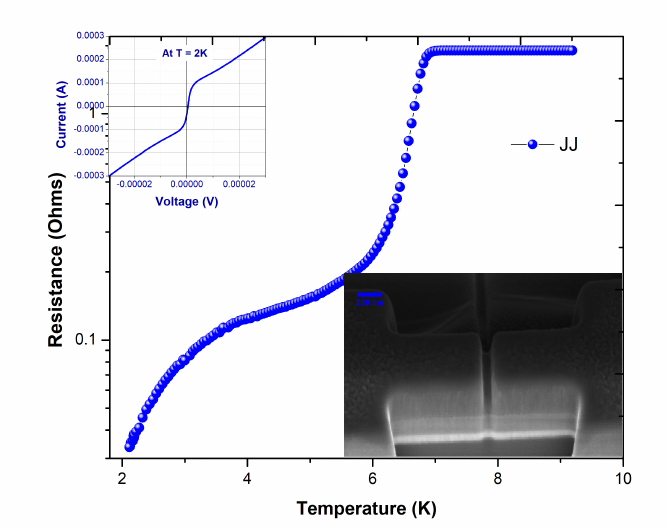
\includegraphics[width=10cm]{JJ}\caption{RT graph for a Cu(100nm)Nb(150nm) Josephson junction. The inset shows
an SEM image of the measured JJ \label{fig:RT-graph-for}}
\end{figure}
The first transition indicates the superconducting transition of the
Niobium layer, and the second transition explains the proximitisation
of the weak link. The resistance $R_{n}$ at 9K (above $T_{c}$) and
$R_{L}$at 2K are noted and the sample is cooled back to sub 2K. $R_{n}$is
the normal resistance and indicates that the device is out of the
superconducting regime. Once the devices cool down to 2K the current-voltage
characteristics of the device is measured by sweeping current from
-$I_{n}$ to +$I_{n}$, where $I_{n}$ is the current for which the
device yields the resistance $R_{n}$ at 2K, ie. the device switches
to the normal regime. The I-V curves have the typical JJ/SQUID behaviour
and is plotted in Fig \ref{fig:IV-graph-for}.
\begin{figure}[H]
\includegraphics[width=10cm]{\string"IV Pt20 CuNbJJ 2k\string".eps}\caption{IV graph for a Cu(100nm)Nb(150nm) Josephson junction \label{fig:IV-graph-for}}
\end{figure}
 $I_{c}$ of the device and the electrodes were extracted from this
data by running through a python script that takes in the I-V data,
calculates dV/dI, and applies a Savitzky--Golay filter of first-order
to obtain $d^{2}I/d^{2}V$ and find the current ($I_{c}$) for which
$d^{2}I/d^{2}V$ in both the positive and negative side and averages
them. For normal Josephson junction the position of peak of $dI/dV$
is a good marker of the $I_{c}$, however in cases where the junction
resistance is high, $dI/dV$ might not be clear enough to mitigate
this peaks of $d^{2}I/d^{2}V$ is a better marker of $I_{c}$ A sample
graph of $dI/dV$ and $d^{2}I/d^{2}V$ for a I vs V curve measured
on a Josephson junction is shown in Fig \ref{fig:findIc}.
\begin{figure}[H]
\centering{}\includegraphics[width=10cm]{samplePlot}\caption{A sample graph of $dI/dV$ and $d^{2}I/d^{2}V$ for a I vs V curve
measured on a Josephson junction. The $I_{c}$ extracted from the
graph is 140$\mu A$ \label{fig:findIc}}
\end{figure}
 The code for the python script is available \href{https://github.com/iamashwin99/JJ-Ic-finder}{here}
and a web app based on the same is hosted at \href{https://jj-ic-finder.herokuapp.com/}{jj-ic-finder.herokuapp.com}

In Fig \ref{fig:IV-graph-for} the IV curve of a Nb/Cu Josephson Junction
is shown. Once the device $I_{c}$ is found, the device is cooled
to 2K and then supplied with $I_{c}$ current, and the junction voltage
is measured while ramping the magnetic field from +250 Oe to -250
Oe ( positive cycle ) and then from -250Oe to 250Oe ( negative cycle
) at 2K. This gives us magnetoresistance as a function of the applied
magnetic field. The magnetoresistance as a function of applied magnetic
field is expected to have a diffraction pattern for JJs and SQUID
oscillations imposed on top of the diffraction pattern for SQUID device
as can be seen in Fig \ref{fig:V-H-graphSQUID} and Fig \ref{fig:V-H-graphSQUID-1}.
This was explained in the theoretical sections above.

\begin{figure}[H]
\includegraphics[width=10cm]{\string"Squid VH\string".eps}\caption{V H graph for a Cu(100nm)Nb(150nm) SQUID, SQUID oscillations and Fraunhofer
pattern can be seen\label{fig:V-H-graphSQUID}}
\end{figure}

\begin{figure}[H]
\includegraphics[width=10cm]{Squid-Oscilations}\caption{Zoomed in graph of V H for a Cu(100nm)Nb(150nm) SQUID, The SQUID oscillations
can be seen clearly\label{fig:V-H-graphSQUID-1}}
\end{figure}

\begin{figure}[H]
\includegraphics[width=10cm]{\string"VH CuNbJJ 2k\string".eps}\caption{Magnetoresistance of the patterned Nb/Cu Josephson junction device
in low magnetic fields for different values of junction currents\label{fig:Magnetoresistance-of-the}}

\end{figure}

\begin{figure}[H]
\includegraphics[width=10cm]{\string"JJ VH\string".eps}\caption{Magnetoresistance of the patterned Nb/Cu Josephson junction device
in low magnetic fields\label{fig:Magnetoresistance-of-the-1}}
\end{figure}

In Fig \ref{fig:Magnetoresistance-of-the-1} , we examine the magnetoresistance
of the patterned Nb/Cu Josephson junction device in low magnetic fields
(|H| < 300 Oe) and at its $I_{c}$. We find that the main lobe of
the positive and the negative cycle overlap completely and there is
no shift of the main lobe from origin as one would expect for a normal
S-N-S junction. Fig \ref{fig:Magnetoresistance-of-the} is a plot
of Junction voltage as a function of magnetic field for another patterned
Nb/Cu Josephson junction device in low magnetic fields for different
values of junction currents. Once can observe that higher currents
increase the height of the lobes however the ratio of the first (main)
lobe to the second lobe remains constant.

\section{Discussion and Conclusion}

We were able to successfully fabricate vertical and planar Nb/Cu Josephson
junctions and through its R-T, I-V, V-H signatures verified that the
device works as expected. The R-T graph shoved the superconducting
transition of the Niobium electrodes sub 7K and slow proximitisation
of the weaklink thereafter. The I-V graph clearly shows the presence
of a critical current $I_{c}$ beyond which the junction behaves resistively,
the $I_{c}$ extraction was automated by analysing the second derivative
of voltage with respect to applied current via a python script. The
VH graph for Josephson junctions shows clear Fraunhofer like pattern
and SQUID oscillations on top of Fraunhofer in the case of SQUIDs
thus further confirming the quality of device thus formed. Future
direction of the project would be to explore alternative materials
for the weaklink of the Josephson junctions. Preliminary literature
survey suggest that 0--$\pi$ oscillations in Superconductor/Ferromagnet/Superconductor
junctions with varying thickness of Ferromagnet layer\cite{sfs-2ndharmonics}.
$\phi$ Josephson junctions are seen with topological insulator $Bi_{2}Se_{3}$
\cite{bi2se3}or 2DEG formed at the surface of InAs layer\cite{InAs-Phasebattery}.
$\phi$ junctions are also observed in weaklinks with high spin orbit
coupling. Further studies on the properties of such weaklinks might
be carried out.

\newpage{}

\bibliographystyle{ieeetr}
\addcontentsline{toc}{section}{\refname}\nocite{*}
\bibliography{report}

\end{document}
